\documentclass[../main.tex]{subfiles}
\begin{document}

\chapter{Solcellesystem} \label{Chap:Solcellesystem}

\section{Batteri}

    \subsection{Designovervejelser}

\section{Maximum Power Point Tracking}

    \subsection{Introduktion}

    For at sikre kontinuerlig maksimal effekt fra solcellen anvendes et MPPT-system til at overvåge for varierende forhold og optimere systemet i realtid. Et MPPT-system gør det muligt hele tiden at opnå den størst mulige effekt fra solcellen, således at så lidt effekt som muligt går til spilde. Systemet er blevet realiseret med en Arduino, der overvåger udgangen fra solcellen og genererer et PWM-signal til en buck-konverter som derved kan justere spænding og strøm for at opnå det optimale forhold. 

    \subsection{MPPT algoritme}

    For at opnå maksimalt energiudbytte fra solcellen benyttes en MPPT-algoritme, som er blevet implementeret på en Arduino ATMEGA2560. Algoritmen har til formål at overvåge solcellesystemet ved at måle effekten fra solcellen, finde det maksimale effektpunkt og levere et passende PWM-signal til en buck-konverter. Der er mange forskellige typer algoritmer til at optimere energiudbyttet fra en solcelle, og i dette projekt er der taget udgangspunkt i en P&O (Perturb & Observe)-algoritme, som er blevet modificeret en smule.

    Arduionen modtager ADC-målinger fra solcellen, som består af en strømmåling og en spændingsmåling fra et analogt kredsløb. Ud fra dette beregner programmet effekten, husker den forrige effektværdi og finder forskellen mellem dg em. På denne måde er det muligt hele tiden at spore, hvilken vej effekten bevæger sig, og korrigere duty-cyclen på PWM-signalet til at ligge omkring et arbejdspunkt for maksimal effekt, som bruges af buck-konverteren. Algoritmen afviger fra den originale P&O-algoritme ved ikke direkte at se på forskelle i spændingsmålinger og derudover have en variabel til at skifte retning på, hvor PWM-signalet bevæger sig hen afhængig af dens placering på den karakteristiske effektgraf for solcellen (vis graf?). Et flowchart for algoritmen er vist i figur \ref{fig: MPPT Flowchart}.  PWM-signalets brug er videre forklaret i afsnittet "MPPT buck".

    \begin{figure}[H]
      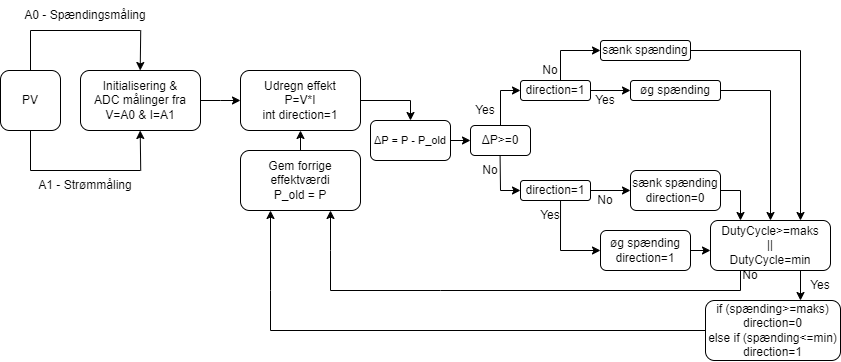
\includegraphics[width=\textwidth]{Dokumentation/mpptflowchart.drawio (1).png}
     \caption{MPPT-algoritme flowchart}
     \label{fig: MPPT Flowchart}
     \end{figure}
    
    Undervejs er der blevet lavet mange ændringer i algoritmen og opsætningen af de forskellige elementer, der bruges i programmet. Vi er stødt på mange udfordringer mht. opsætning og behandling af analoge måleværdier, timere og generel stabilitet af systemet og har måttet bruge en del tid på at overkomme disse problemer. Der er til sidst i projektet fundet en effektiv løsning, som giver os den ønskede effekt af et MPPT-system.

    MPPT-koden er vedhæftet som bilag.


    \subsection{MPPT buck}
        Dette delkredsløb kontrolleres af MPPT-algoritmen og anvendes til at regulere indgangsstrøm/spændingen fra solcellen så effekten kan tilpasses og optimeres efter det påsatte load.
        
        \subsubsection{Delkrav}

            \begin{enumerate}
                \item Skal kunne regulere forholdet mellem sin egen indgangs- og udgangsspædning samt indgangs-/udgangsstrøm som en funktion af et PWM-kontrolsignal.
                \item Skal kunne håndtere en indgangspændning på op til 23V
                \item Skal kunne håndtere en indgangsstrøm på op til 0.66A
                \item Må ikke trække mere end 20 mA fra PWM-signalet.
                \item Skal være effektiv nok til at tillade videre regulering af udgangsspændingen til 5V og herefter kunne oplade en kondensator.
                \item Skal kunne fungere ved 50kHz.
            \end{enumerate}
            
        \subsubsection{Designovervejelser}
            
            
            Switch
            I valg af switch overvejes forskellige opsætninger af switches som vist i figur \ref{fig: Switch designs}. I figuren ses de forskellige iterationer af switch opsætninger der er blevet anvendt i buck converterne i PV-delen af opsætningen. Figuren viser den første iteration af switch længst til vænstre og nyere versioner mod højre.
            \newline
            I iteration 3 anvendes opsætningen som er lavet til en P-kanal med en N-kanal MOSFET. Dette skyldes problemer med den valgte P-kanal mosfet i iteration 2 af valg af switch. Det skal noteres at selv om denne opsætning af switch er den der indgår i den endelige opsætning er dette ikke en optimal løsning da Gate-Source ON spændingen vil føre til et spændingstab på ca. 2 volt over MOSFET'en. Grundet tidsmangel er en mere optimeret opstilling som den set i iteration 4 ikke blevet implementeret.\newline
            
            \begin{figure}[H]
            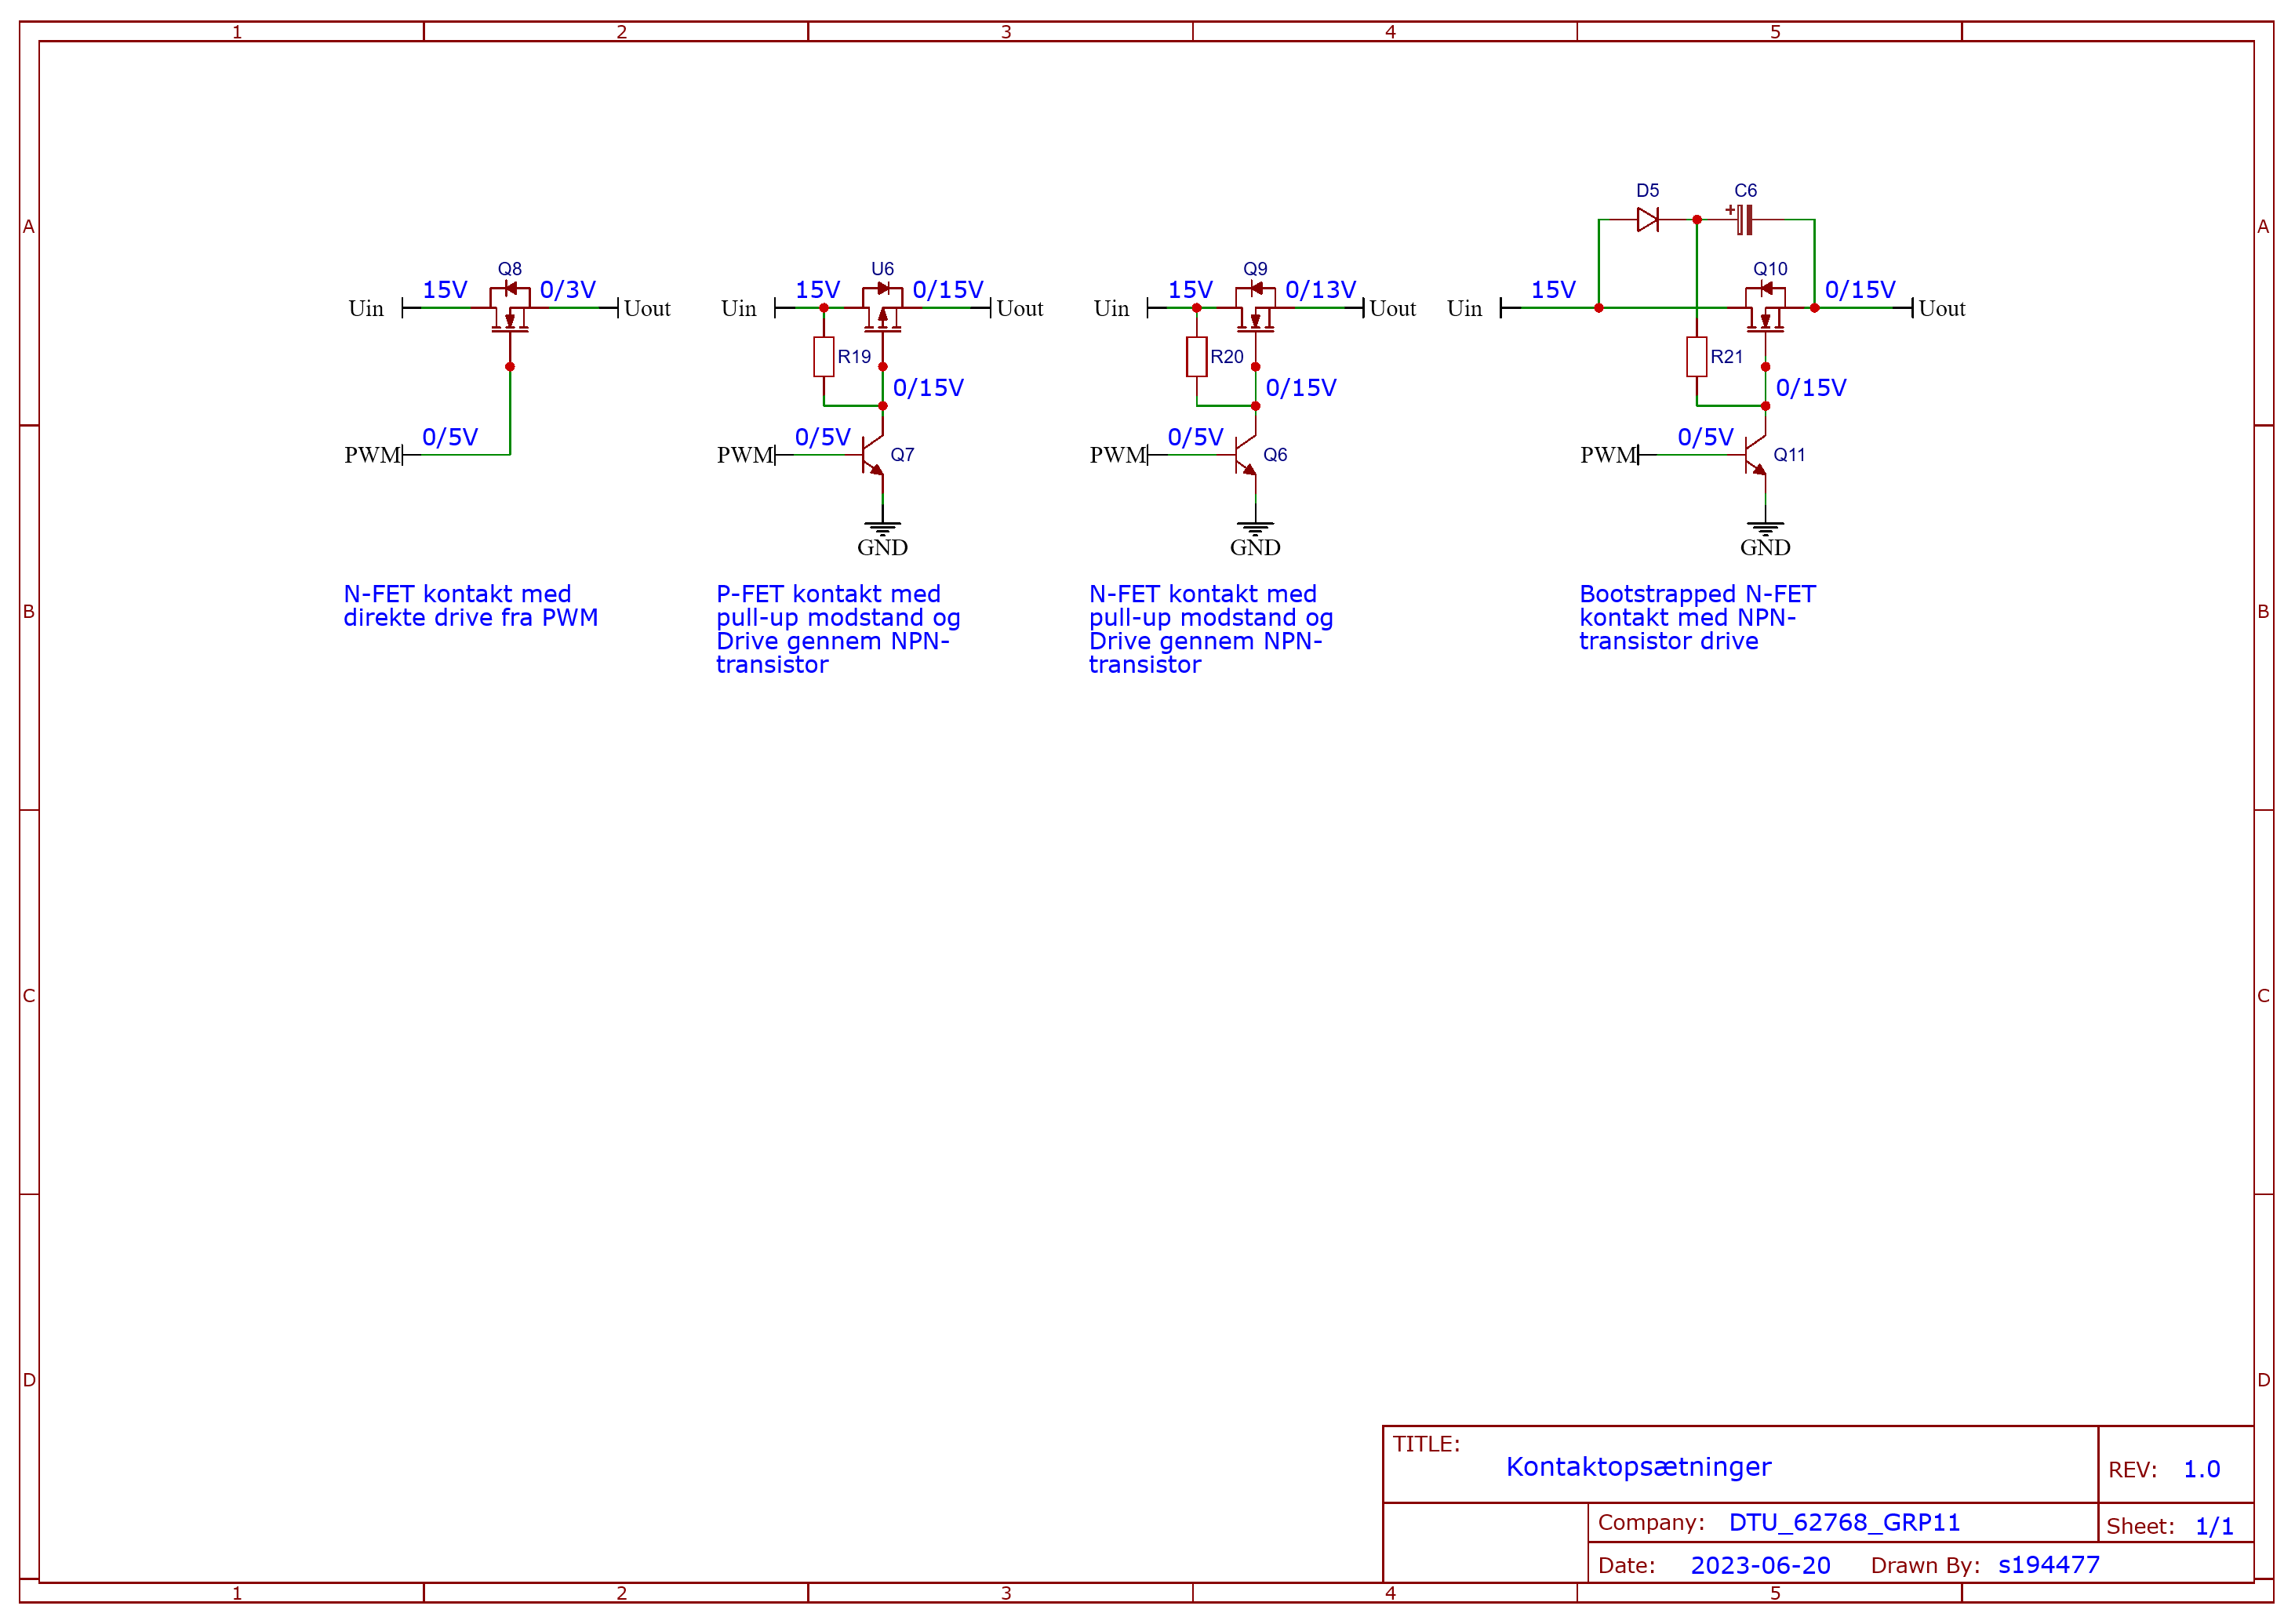
\includegraphics[width=\textwidth]{Dokumentation/Figures/PV_Converter switches.png}
            \caption{Forskellige itterationer af switch-opsætninger til buck convertere.}
            \label{fig: Switch designs}
            \end{figure}
            
            filterkomponenter:
                Følgende ligning beskriver den teoretiske udgangspænding af en buck converter i forhold til dens indgangsspænding:\newline
                $$U_{ud} = PWM \cdot U_{ind} $$\newline
                Det fremgår af dette at den gennemsnitlige udgangsspænding ikke er afhængig af filterværdierne beskrevet i følgende.
            
        \subsubsection{Implementering}

            Kondensator:
            Det fremgår af det overordnede diagram i projektbesrkivelsen (se appendix \ref{}) at der mellem MPPT'en og 5volts reguleringen i PV-grenen skal indgå en ladekondensator med en komponentværdi på 15mF. For simplificering af kredsløbbet implementeres denne ved at anvende denne kondensator som filterkondensator og denne værdi er derfor givet.
            
            Spole
            I valg af spole tages højde for at denne har en minimumsvørdi for at kunne køre i en kontinuert operationscyklus. Herudover har spolens værdi inflydelse på størelsen af de fluktiationer der ses i udgangsstrømmen, $\Delta I$.\newline

            Spoleværdien kan estimeres ud fra følgende ligning:
            $$L = \frac{1-k}{16 f^2 C}$$
            $$\rightarrow L = \frac{1-0}{16\cdot 50\cdot 10^3 Hz \cdot 15\cdot 10^{-3}F} \rightarrow 1,33nF$$
            \newline
            Ved denne værdi vil udsvingene i udgangstrømmen dog være for stor. Af denne årsag vælges en støre spoleværdi hvor den maksimale udsvinging ikke overgår 2\% af solcellens udgangsstrøm ved maksimal effekt.
            $$\Delta I_{2\%} = 0,02 \cdot I_{MP} = 0,02 \cdot 0,66A = 13,2mA$$
            $$L = \frac{U_s(1-k)k}{f\cdot \Delta I} = \frac{15 V\cdot (1-0,2)\cdot 0,2}{50\cdot 10^3 Hz \cdot 13,2 \cdot 10^{-3} A} = 3,64mH$$\newline
            
            
            Diode
            En Shotky diode tænkes at anvendes da disse har et lavere fremadrettet spændingsfald. Dette bør føre til en højere effektivitet, og en sådan diode forsøges derfor at vælges i implementeringen.
            
            
        \subsubsection{Test}
            
            
            
            
        \subsubsection{delkonklusion}
            
            
            
            
    \subsection{MPPT strøm/spændingsmåler}
            
        \subsubsection{Delkrav}
            
        \subsubsection{Designovervejelser}
            
        \subsubsection{Implementering}
            
        \subsubsection{Test}
            
        \subsubsection{delkonklusion}
            
            
                    
\section{Udgangsconverter}
        
    \subsection{Delkrav}
        
    \subsection{Designovervejelser}
            
            Switch

            Spole

            Kondensator

            Diode


            
    \subsection{Implementering}
        
    \subsection{Test}
        
    \subsection{Delkonklusion}
        
        
\end{document}